\documentclass[a4paper,12pt]{article}
\usepackage{color}
\usepackage{graphicx}
\usepackage{hyperref}
\usepackage{float}
\usepackage{rotating}

\begin{document}
\title{Dokumentation}
\author{Radike, Sauer, Wolf}
\date{\today}
\maketitle

\begin{tabular}[h]{l|l|l|l} %l = left c = center r = right
	Version & Datum & Autor & Änderung/Bemerkungen\\
	\hline\hline
	1.0 & 11.02.2021 & Sauer Lukas & Erstellung\\
	\hline
	1.1 & 25.02.2021 & Sauer Lukas & intADC\\
	\hline
	1.3 & 18.03.2021 & Sauer Lukas &  Vorwort \& ADC-PCB \& ext. ADC\\
	\hline
	2.0 & 08.04.2021 & Sauer Lukas &  Kommunikationsprotokoll\\
	\hline
	2.1 & 15.04.2021 & Sauer Lukas &  update Kommunikationsprotokoll\\
	\hline
	3.0 & 15.04.2021 & Sauer Lukas &  Trigger\\
\end{tabular}
\newpage
\tableofcontents
\newpage

\section{Vorwort}

\subsection{Projektübersicht}
Im Projekt Oszi wird ein Oszilloskop mittels eines FPGAs zu realisieren. Das Oszilloskop soll ein Frequenzband von 0Hz bis 500kHz einlesen und einen Spannungsbereich von -20V bis +20V abdecken. Die Spannungskurfe soll über ein Computerprogramm graphisch ausgegeben werden. Über das Programm soll ebenfalls der Spannungs- und Zeitbereich der Ausgabe einzustellen sein. Das Oszilloskop solle triggerbar sein und Tastköpfe kalibrieren können. Das Projekt besteht aus drei Aufgabenbereichen, dem Analog-Front-End, der Datenverarbeitung mit dem FPGA und der Ausgabe am PC.
\subsection{Projektgruppe}
Das Team entstand im Zuge des Sommersemster-Projekts in der 4. Schulstufe am TGM. Gleiche Intressen, gutes technisches Wissen und Verständnis, sowie eine gute Harmonie unter den Fruppenmitgliedern führte zum Zusammenschluss. Die Projektgruppe ist geschlossen aus einer Klasse, der 4AHEL 2021 am TGM.
\begin{center}
\begin{tabular}[h]{c|c|c}
\multicolumn{3}{ c }{Projektteilnehmer}\\
\hline
\textbf{Radike} & \textbf{Sauer} & \textbf{Wolf}\\
Markus & Sauer & Benedict\\
\hline
Bild 1 &  \raisebox{-\height}{
\includegraphics[width=4cm]{Vorwort/FotoSauer.jpg}} & bild 3\\
\! & \! & \!\\
\hline
user interface & digital data processing & analog front end\\
\end{tabular}
\end{center}

\subsection{Projektbetreuer}
\begin{tabular}[h]{l|l}
		Fachbereich & Lehrperson\\
		\hline\hline
		Labor & GRÄBNER Kar-Heinz\\
		\hline
		Werkstatt & GRAUPE Andreas\\
	\end{tabular}

\section{Entwicklung}
\subsection{Der ADC - LTC1420C}\label{extADC}
 Die Wahl des externen ADCs ist auf den LTC1420C gefallen. Dieser besitzt eine Auflösung von 12-Bit bei einer Abtastrate von 10MSa/s.  Ausgelesen werden die Messwerte vom FPGA parallel über 12 digitale Ausgänge. Der ADC benötigt keine Referezspannung, da diese intern erzeugt wird, jedoch eine Clock von 10Mhz muss bereit gestellt werden.
Das Datenblatt ist in den Quellen verlinkt, siehe \ref{LTC1420C_dat}

\section{verwendete Messgeräte \& Entwicklungstools}
\subsection{DE10-Lite Board} \label{DE10-Lite}
\begin{tabular}[h]{l|l}
	Art & DE-Lite Board\\
	\hline
	Produktnummer & DE10-Lite\\
	\hline
	Seriennummer & 19040005-1757\\
	\hline
	TGM Inv. Nr. & Eigentum Sauer\\
	\hline
	Beschreibung & FPGA-Entwicklungsplatine\\
	& Chip: Max 10 10M50DAF484C7G\\
	& 50 MHz\\
	& Power Supply: 5V USB\\
	\hline
	Foto & \raisebox{-\height}{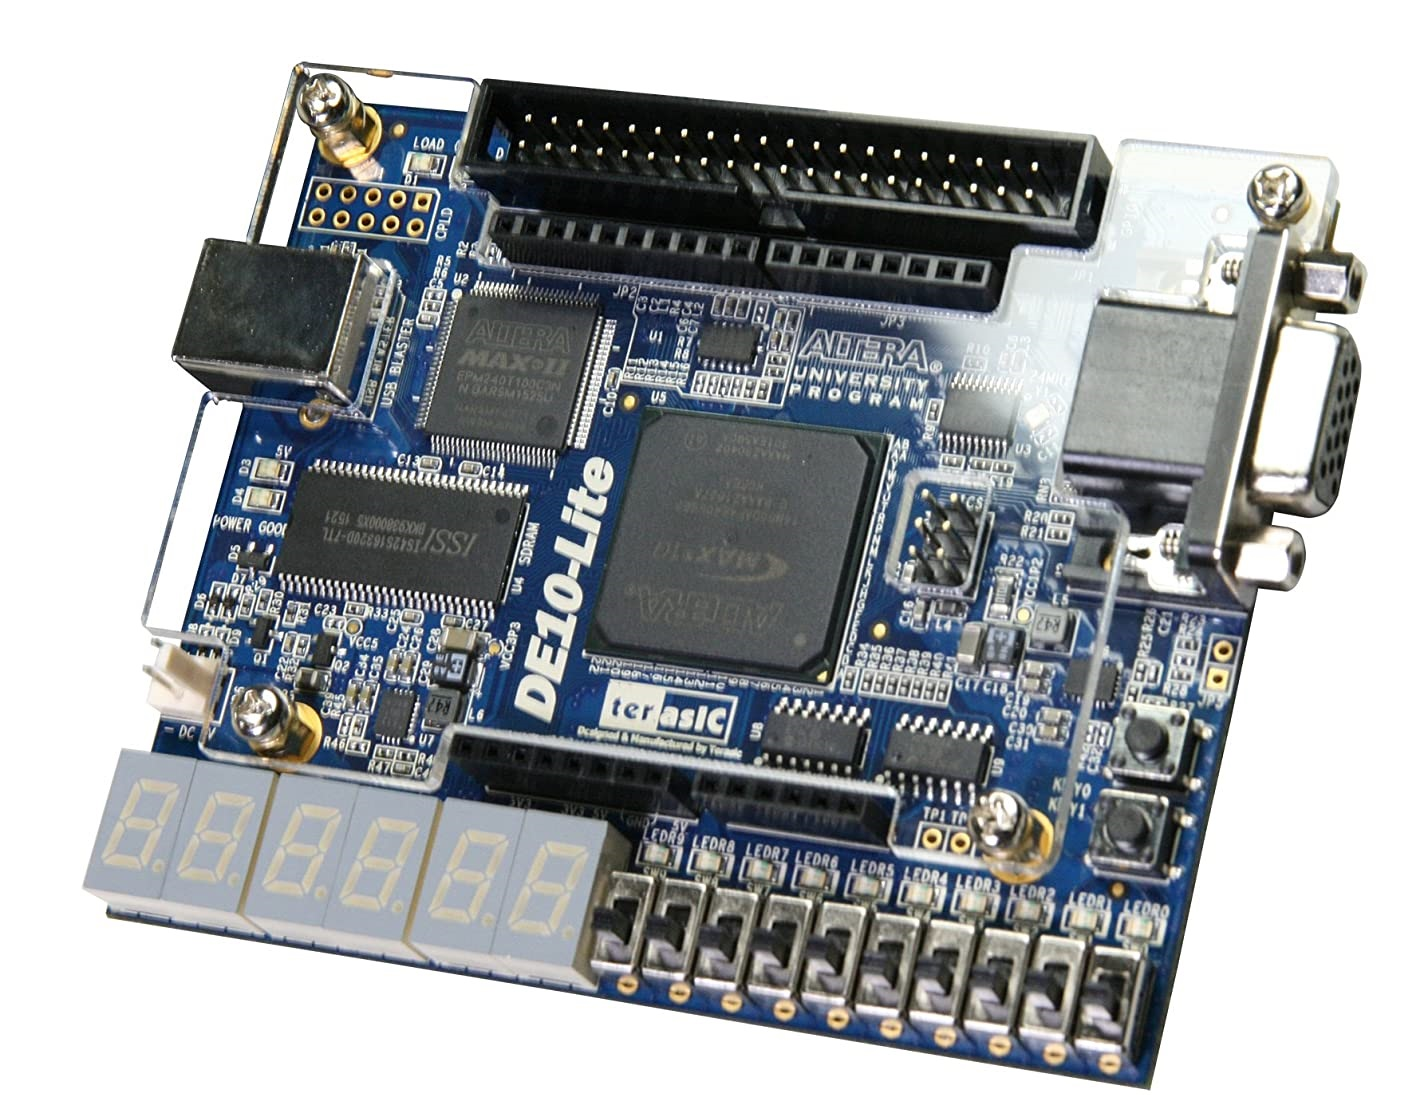
\includegraphics[width=8cm,angle=0]{Geraete/DE10-Lite.jpg}}\\
\end{tabular}
\subsection{Oszilloskop 1} \label{Oszi1}
\begin{tabular}[h]{l|l}
Art & Oszilloskop\\
\hline
Marke & Hameg\\
\hline
Produktnummer & HM1507-2\\
\hline
Seriennummer & /\\
\hline
TGM Inv. Nr. & 540-16/22/99\\
\hline
Beschreibung & digitales Oszilloskop\\
 & 2 Channel\\
 & 150 MHz | 200 MSa/s\\
 & Röhrenbildschirm\\
\hline
Foto & \raisebox{-\height}{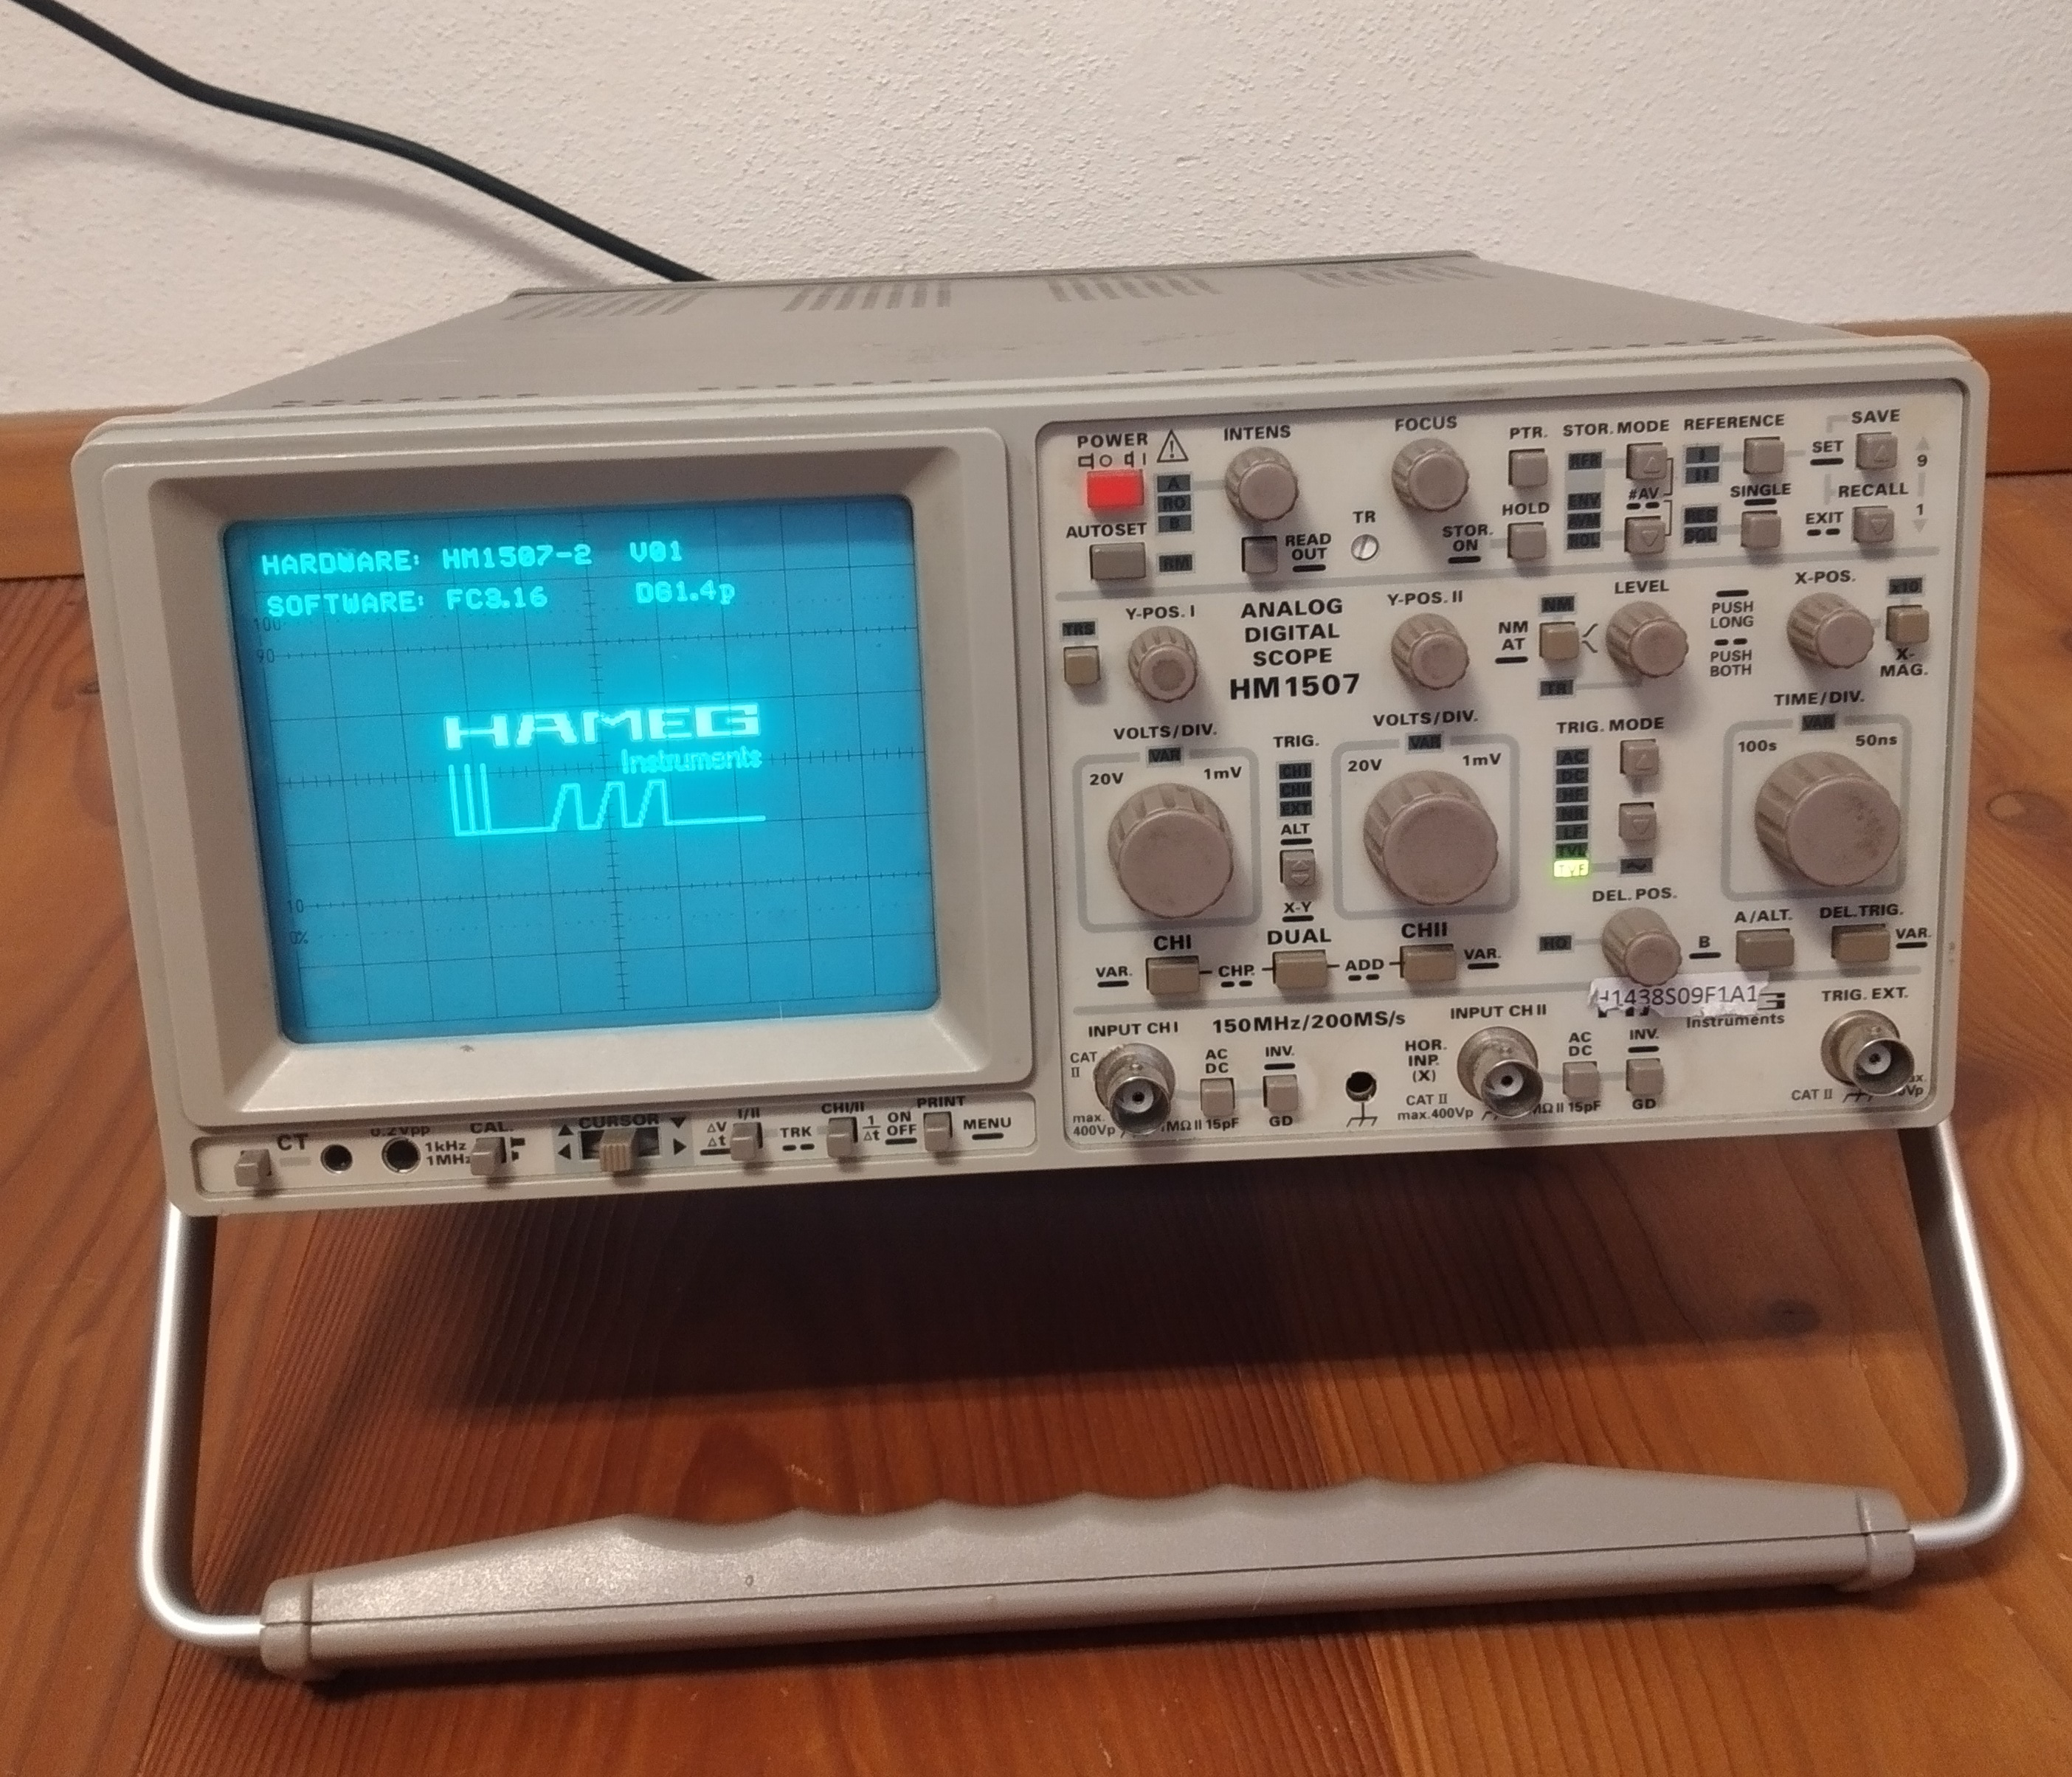
\includegraphics[width=8cm,angle=0]{Geraete/Oszi1.jpg}}\\
\end{tabular}
\subsection{Funktionsgenerator 1} \label{Funktionsgen1}
\begin{tabular}[h]{l|l}
	Art & Funktionsgenerator\\
	\hline
	Marke & HP\\
	\hline
	Produktnummer & H3312A\\
	\hline
	Seriennummer & 1502G00232\\
	\hline
	TGM Inv. Nr. & Eigentum Sauer\\
	\hline
	Beschreibung & analoger Funktionsgenerator\\
	& 1 Channel\\
	& 13 MHz sinus/rechteck/dreieck\\
	\hline
	Foto & \raisebox{-\height}{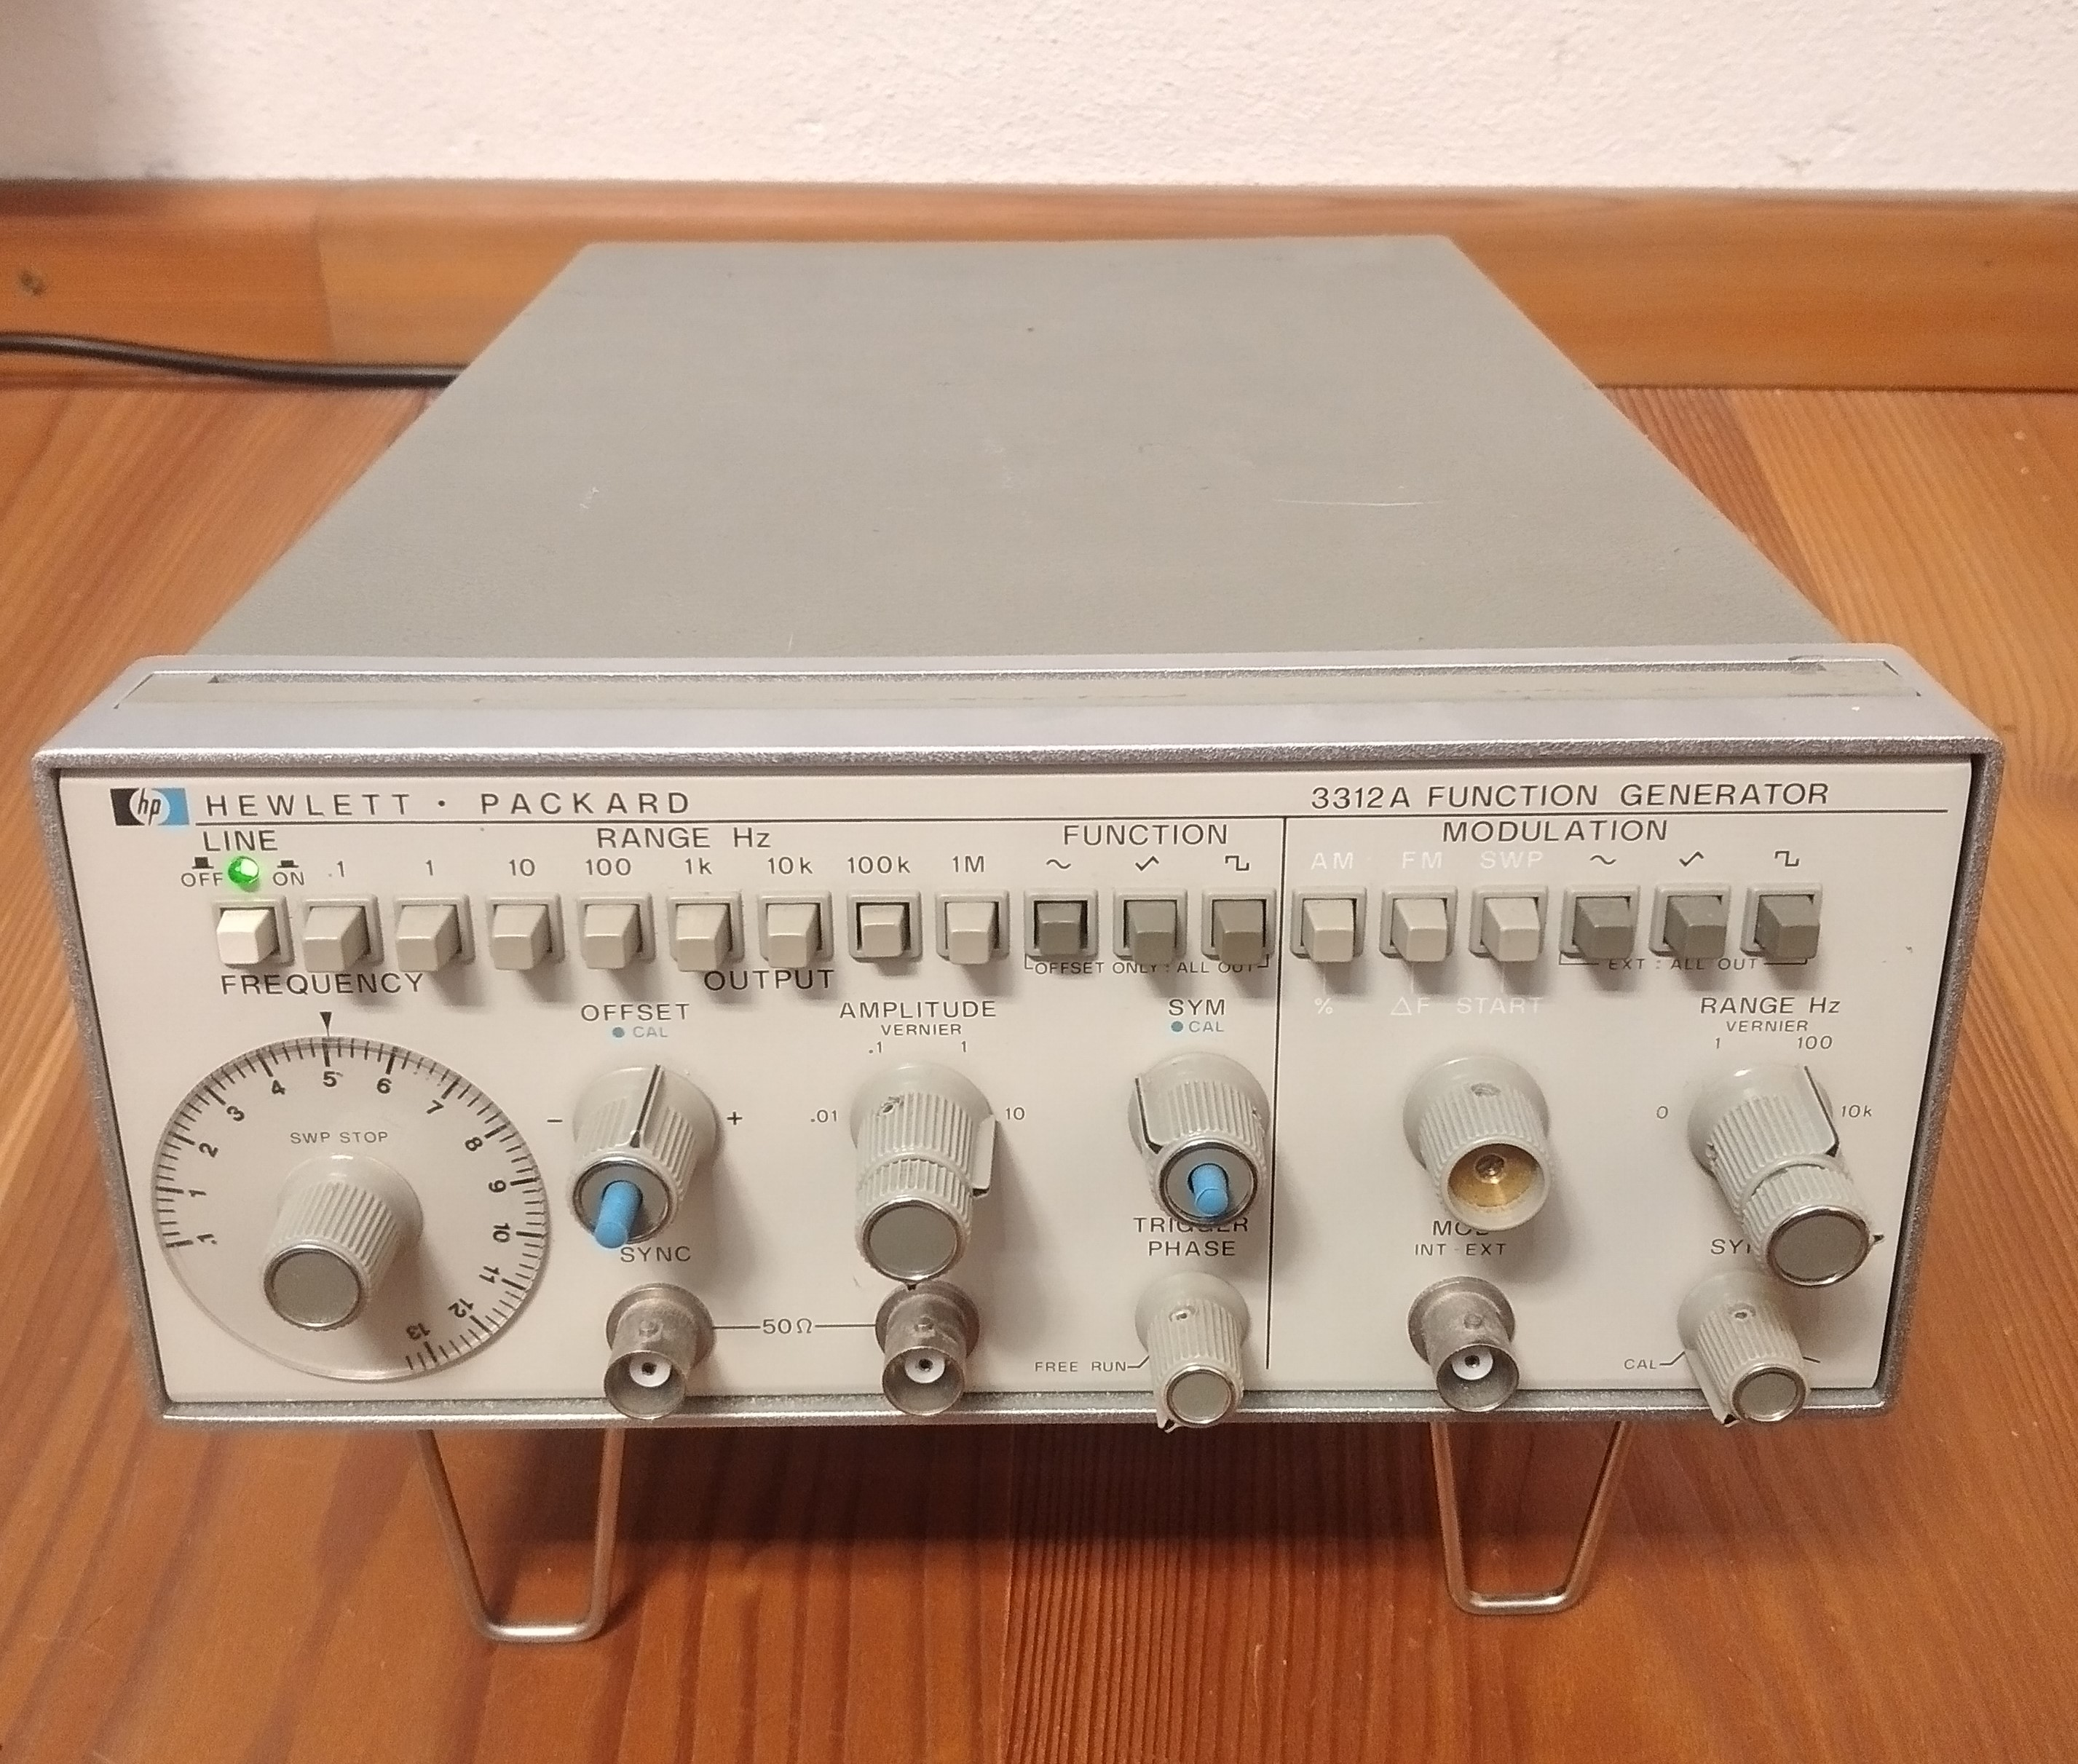
\includegraphics[width=8cm,angle=0]{Geraete/Funktionsgen1.jpg}}\\
\end{tabular}
\subsection{RS232-Adapter} \label{RS232-Adapter}
\begin{tabular}[h]{l|l}
	Art & RS232-Adapter\\
	\hline
	Produktnummer & AU0002E\\
	\hline
	Seriennummer & /\\
	\hline
	TGM Inv. Nr. & Eigentum Sauer\\
	\hline
	Beschreibung & Umsetzter RS232 <-> USB \\
	& DSUB 9 Pin männlich\\
	& USB-A männlich\\
	\hline
	Foto & \raisebox{-\height}{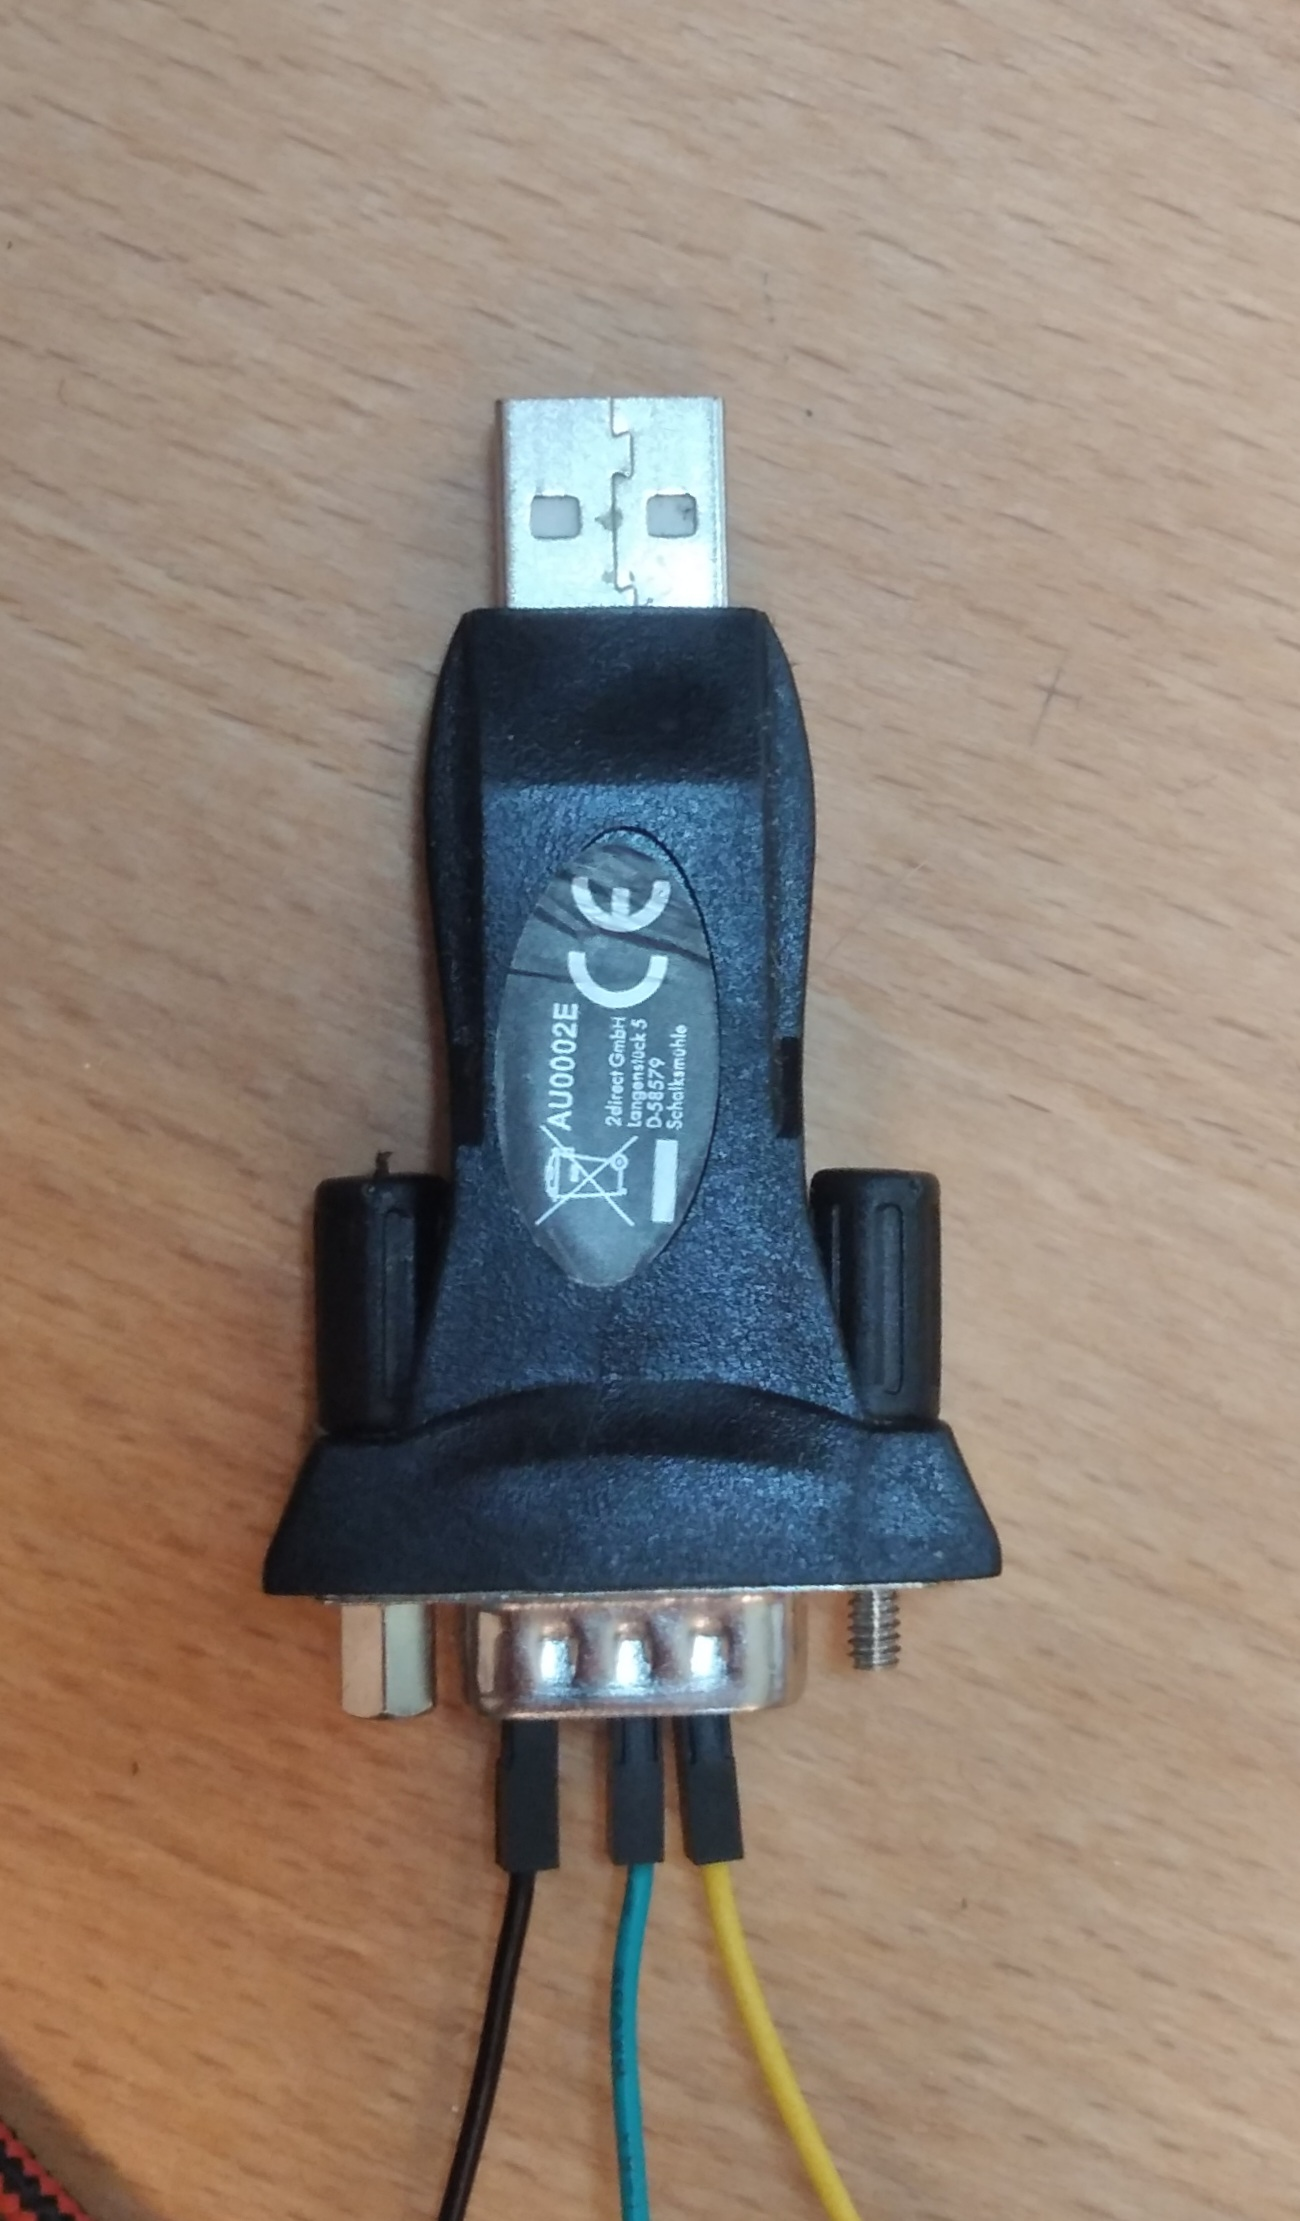
\includegraphics[width=5cm,angle=90]{Geraete/RS232.jpg}}\\
\end{tabular}
\section{Quellen und Hilfsmittel}
\paragraph{Verwendung des DE10-Lite-Boards \& VHDL-Programmierung:}
\begin{itemize}
\item
Übersicht: DE10-Lite-Board: DE10-Lite\_v.2.1.0\_SystemCD: DE10-Lite\_User\_Manual.pdf
\item
\label{Schaltplan_FPGA}
Schaltplan: DE10-Lite-Board: DE10-Lite\_v.2.1.0\_SystemCD: de10-lite.pdf
\item
VHDL-Spezifikation: \url{https://www.nandland.com}
\item
Infos zum Triggern: \url{https://www.tiepie.com/en/fut/edge-trigger}
\item
UART VHDL Code: \url{https://www.digikey.com/eewiki/pages/viewpage.action?pageId=59507062}
\end{itemize}
\paragraph{Datenblätter:}
\begin{itemize}
\item \label{LTC1420C_dat}
\textbf{LTC1420C:} \url{https://www.analog.com/media/en/technical-documentation/data-sheets/1420fa.pdf}
\end{itemize}
	

\end{document}